\chapter{Résultats}

Préalablement aux résultats acquis durant le stage, plusieurs étapes de mises
au point (notamment sur lignées cellulaires de plasmocytes et échantillons de
\gls{llc}) ont été réalisées durant l'année 2024-2025. Les données ne seront
pas présentées dans ce rapport, mais ont permis de valider la faisabilité de
l'analyse des réarrangements \gls{vdj} via le protocole précédement décrit,
sous-tenant quelques modifications, mais aussi de faire la lumière sur
plusieurs difficultés.

\section{Limites et contraintes du protocole FR3}

\subsection{Identification incertaine du segment V}

Une des premières difficultés rencontrées, inhérente à la nature du protocole
utilisé, est l'incertitude sur l'identification du segment V. En raison de
l'utilisation d'amorces ciblant la région \gls{fr}3, toujours dans l'optique
d'analyser par la suite des \gls{adnc}, seuls 20 à 30 nucléotides sont
séquencés en amont du réarrangement \gls{vdj}. Cette longueur ne permet pas à
\textit{Vidjil} (ou tout autre outil d'analyse de réarrangements \gls{vdj}) de
déterminer avec certitude le segment V utilisé (\autoref{fig:v-leader-fr3}).
Une façon de remédier à ce problème est de d'amplifier au diagnostic en
utilisant des amorces ciblant la région \gls{fr}1 ou \textit{leader}, pour
obtenir une séquence plus longue, et ainsi permettre à \textit{Vidjil} de
déterminer le segment V utilisé. L'unicité de la région \gls{cdr}3 permettra
ensuite de relier les clones identifiés sur les prélèvements de suivi.

\begin{figure}[H]
    \centering
    \begin{ttfamily}
        \begin{tabular}{@{}l@{}}
            \textbf{Clone IGHV1-3*04 // D3-16 // J3*02 (\textit{leader})}                                      \\
            \colorbox{blue!20}{GCCAGGCCCCCGGTCAGAGGCTTGAGTGGATGGGCTGGGTCAACGGTGCCAGTGGCGACGCAAAATATTCACAGCAT}  \\
            \colorbox{blue!20}{TTCCAGGGCGGAGTCACCATTACCAGGGACACTTCCGCGACTACAGCCTACATGGAACTGAGCAGCCTGAGATCTGAG} \\
            \colorbox{blue!20}{GACACGGCTGTCTATTACTGTGCGA}%
            \colorbox{green!20}{CTTATACC}AACACTTTTTGGTT%
            \colorbox{orange!20}{TGCTTTTGATATCTGGGGCCAAGGGACAA}                                                \\
            \colorbox{orange!20}{TGGTCACCGTCTCCTCAG}GT                                                         \\
            \\
            \textbf{Clone IGHV3-30*08 // D3-16 // J3*02 (\gls{fr}3)}                                           \\
            \textbf{
                \textcolor{red}{\faExclamationTriangle\  Gènes V équiprobables : IGHV3-66*02, IGHV3-7*02, IGHV3-30*08, IGHV4-34*12}
            }                                                                                                  \\
            \colorbox{blue!20}{GACACGGCTGTCTATTACTGTGCGA}%
            \colorbox{green!20}{CTTATACC}AACACTTTTTGGTT%
            \colorbox{orange!20}{TGCTTTTGATATCTGGGGCCAAGGGACAA}                                                \\
            \colorbox{orange!20}{TGGTCACCGTCTCCTCAG}GT
        \end{tabular}
    \end{ttfamily}
    \caption{Alignement de deux réarrangements clonaux identiques. Le premier clone (en haut) correspond à un réarrangement
        complet séquencé en \textit{leader}, tandis que le second (en bas) commence au niveau de la région \gls{fr}3.
        Les séquences en \colorbox{blue!20}{bleu} correspondent au segment V, en \colorbox{green!20}{vert}
        au segment D, et les séquences en \colorbox{orange!20}{orange} correspondent au segment J.
        }
    \label{fig:v-leader-fr3}
\end{figure}

\subsection{Impact de l'hypermutation somatique sur l'amplification}

Il s'agit encore une fois d'une difficulté liée au protocole d'amplification
\gls{fr}3 et à la nature des cellules d'interêt. En effet les plasmocytes
constituent le stade le plus mature de la lignée lymphoïde B, et en ce sens
sont donc les cellules où le réarrangement \gls{vdj} comporte le moins
d'homologie avec les séquence germinales. La conséquence de ceci étant que dans
certains cas, les amorces utilisées pour l'amplification \gls{fr}3 ne sont pas
capables de se fixer sur les séquences \gls{vdj} mutées, et amplifier les
réarrangements. L'utilisation d'amorces dégénérées permet de limiter ce
problème sans le résoudre totalement pour autant. Dans le cas où le
réarrangement \gls{vdj} n'est pas amplifiable, il est possible d'analyser en
lieu les réarrangements incomplets DH-JH (cf \autoref{fig:vdj}). Ainsi en guise
d'illustration, parmi les 5 patients analysés, le patient 1 présente un
réarrangement amplifié en \gls{fr}3, tandis que chez le patient 2, le
réarrangement n'est pas amplifié (\autoref{fig:primer-alignement}).

\begin{figure}[H]
    \centering
    \begin{ColoredVerbatim}
                10         20 
        \G\Hbase\G\G\A\C\A\C\N\G\C\Y\G\T\G\T\A\T\T\A\C amorce dégénérée VH commune
        \textcolor{gray}{|:||||||:||:|||||||||}
        \G\A\G\G\A\C\A\C\G\G\C\T\G\T\G\T\A\T\T\A\C séquence IGHV3-30 patient 1
           150       160

                10        20 
        \G\Hbase\G\G\A\C\A\C\N\G\C\Y\G\T\G\T\A\T\T\A\C amorce dégénérée VH commune
        \textcolor{gray}{ :|||| |:| :   ||||||}
        \A\T\G\G\A\C\Tb\C\A\G\G\C\A\C\Tb\T\A\T\T\A\C séquence IGHV2-5*04 patient 2
              160       170
    \end{ColoredVerbatim}
    \caption{
        Alignement de l'amorce dégénéree VH commune utilisée pour l'amplification \gls{fr}3 
        avec les séquences V majoritaires identifiées chez les patients 1 et 2 en \textit{leader}. 
        Un alignement est représenté par | et : pour les nucléotides dégénerés. Les bases soulignées 
        correspondent aux bases mutées par rapport à la séquence germinale.
    }
    \label{fig:primer-alignement}
\end{figure}

\subsection{Amplification non spécifique et artefacts de PCR}

Un dernier problème, et non des moindres, concerne l'amplification non
spécifique de régions non ciblées par les amorces, ainsi que la présence de
nombreux artéfacts dans les données de séquençage. Les amorces utilisées
faisant de l'ordre de 100 bases (cf \autoref{anx:primer-sequences}), elles ont
tendance à se dimériser et ainsi être amplifiées et séquencées en l'état. De
plus, certaines amorces, notamment celle ciblant la région JH commune,
amplifient des régions non ciblées dans les conditions actuelles de \gls{pcr}.
Pour illustrer, chez le patient 1 sur le même prélèvement au diagnostic, on identifie 
un clone majoritaire qui represente près de 82 \% des clones identifiés en \textit{leader}, 
contre 32 \% en \gls{fr}3 au milieu de nombreuses séquences artéfactuelles et hors-cibles 
\footnote{Traduction un peu libre de l'anglais \textit{off-target}} (\autoref{fig:fr3-vs-leader}).

\begin{figure}[H]
    \centering
    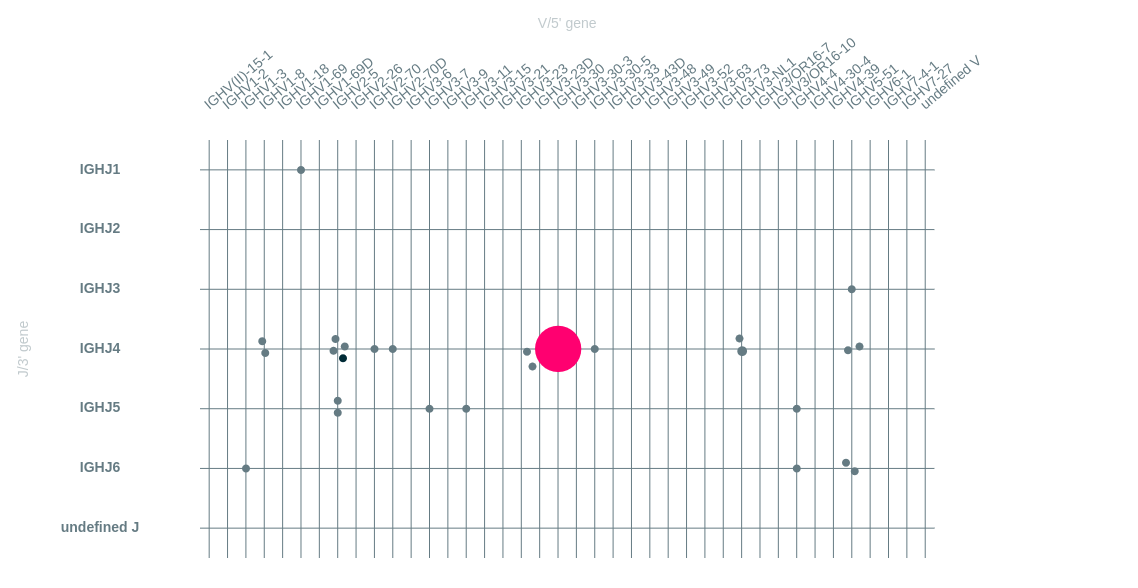
\includegraphics[width=1\textwidth]{images/diag_leader.png}
    \vspace{0.5cm}
    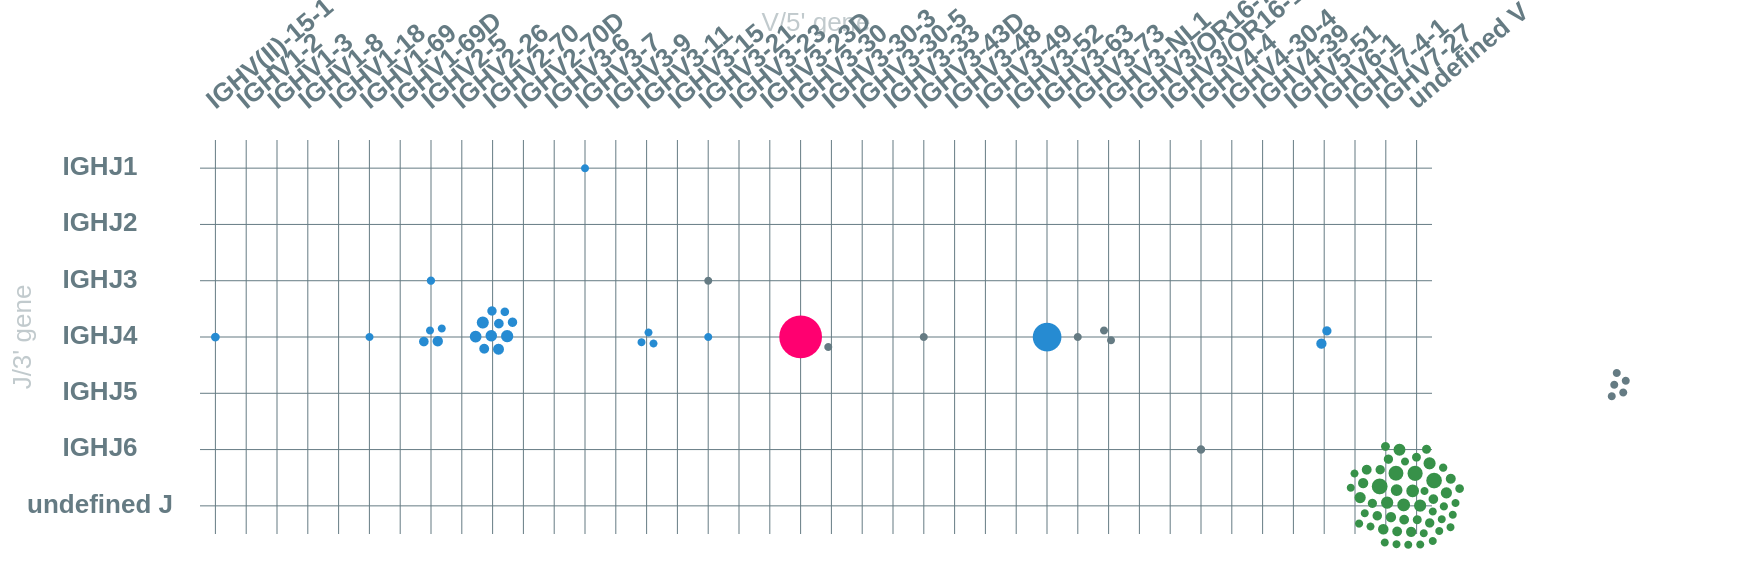
\includegraphics[width=1\textwidth]{images/diag_fr3.png}
    \caption{
        Répartition des clones identifiés en \textit{leader} (en haut) et en \gls{fr}3 (en bas)
        pour le patient 1 au diagnostic. On observe que le \textcolor{Magenta}{clone majoritaire (en rose)}
        en \textit{leader} devient plus minoritaire en \gls{fr}3, devant les \textcolor{ProcessBlue}{nombreux clones artéfactuels (en bleu)}
        et \textcolor{ForestGreen}{hors-cibles (en vert)}.
    }
    \label{fig:fr3-vs-leader}
\end{figure}

\section{Optimisations techniques et bioinformatiques}

Un certain nombre des défis posés par le protocole de séquençage \gls{fr}3 ont
pu être surmontés conjointement par des adaptations techniques et
bioinformatiques. Au niveau du protocole d'amplification, une refonte complète
des concentrations relatives des différentes amorces, du protocole d'extration
et des températures de \gls{pcr} ont permis d'améliorer nettement la qualité
des données obtenues. Le cœur de cette section sera consacré au détail des
approches bioinformatiques mises en place, notamment concernant les clones
artéfactuels issus des dimères d'amorces et séquences hors-cibles.

\subsection{Filtrage des séquences hors-cibles}

En ce qui concerne les artéfacts issus des dimères d'amorces, il est assez
naturel que \textit{Vidjil} les identifie comme des réarrangements \gls{vdj}
valides, comprenant une section V ou J. Il est par contre plus surprenant que
des séquences ne comprenant ni gène V ni J soient également identifiées comme
des réarrangements \gls{vdj} valides. Ces séquences étant par ailleurs souvent
majoritaires dans les premières données obtenues, pouvant représenter jusqu'à
50 \% des \textit{reads} identifiés par \textit{Vidjil}.

En y regardant de plus près, ces séquences s'alignent sur diverses régions du
génome, de façon quasi parfaite, à l'exception de quelques bases aux extrémités
des séquences. Ces bases sont toutes identiques et correspondent à la séquence
\C\G\T\C\T\C\C\T\C\A\G\G\T\A\A\G, ou à sa séquence complémentaire (inversée)
\C\T\T\A\C\C\T\G\A\G\G\A\G\A\C\G.

Dans l'hypothèse d'une amplification non spécifique, il est possible que ces
séquences correspondent à des fragments d'amorces, hypothèse qu'il est facile
de vérifier en recherchant ces séquences dans les amorces utilisées pour
l'amplification (\texttt{primers.fa} comprenant les différentes combinaisons de
bases dégénerées) (\autoref{lst:bash-search-primer}).

\begin{lstlisting}[language=custombash, 
caption={Commande Bash et résultat de la recherche des séquences dans les amorces dégénérées.},
label={lst:bash-search-primer},
basicstyle=\ttfamily\scriptsize]
$ grep -i --color -C 1 "CTTACCTGAGGAGACG" primers.fa
>IGH-J-A-1
caagcagaagacggcatacagatxxxxxxxxgtgactggagttcagacgtgtgctcttccgatctCTTACCTGAGGAGACGgtgacc

$ echo "CGTCTCCTCAGGTAAG" | tr 'ACGT' 'TGCA' | rev | \
        xargs -I{} grep -i --color -C 1 {} primers.fa
>IGH-J-A-1
caagcagaagacggcatacagatxxxxxxxxgtgactggagttcagacgtgtgctcttccgatctCTTACCTGAGGAGACGgtgacc
\end{lstlisting}

Ces séquences sont donc issues de l'amorce JH commune, et on peut en déduire le
phénomène suivant : dans les conditions de \gls{pcr} utilisées (notamment de
température), l'amorce JH se fixe à des régions du génome autres que les
régions JH par complémentarité faible, et amplifie ces régions recopiant au
passage la séquence de l'amorce spécifique de la région JH
(\autoref{fig:off-target-amplification}). Ces séquences sont ensuite
identifiées par \textit{Vidjil} comme des réarrangements \gls{vdj} valides
incomplets.

\begin{figure}[H]
    \centering
    \begin{ColoredVerbatim}
        
        NNNNNNNNNNNNNNNNNNNNNNNNNNNNNNNNNNNNNNNN Région quelconque double brin
        NNNNNNNNNNNNNNNNNNNNNNNNNNNNNNNNNNNNNNNN

        NNNNNNNNNNNNNNNNNNNNNNNNNNNNNNNNNNNNNNNN Dénaturation (Cycle 1)

                               \C\G\T\C\T\C\C\T\C\A\G\G\T\A\A\G
        NNNNNNNNNNNNNNNNNNNNNNNNNNNNNNNNNNNNNNNN Fixation de l'amorce JH


        NNNNNNNNNNNNNNNNNNNNNNN\C\G\T\C\T\C\C\T\C\A\G\G\T\A\A\G
        NNNNNNNNNNNNNNNNNNNNNNNNNNNNNNNNNNNNNNNN Amplification

        NNNNNNNNNNNNNNNNNNNNNNN\C\G\T\C\T\C\C\T\C\A\G\G\T\A\A\G Dénaturation (Cycle 2)

                               \C\G\T\C\T\C\C\T\C\A\G\G\T\A\A\G
        NNNNNNNNNNNNNNNNNNNNNNNNNNNNNNNNNNNNNNNN Fixation de l'amorce JH, etc.
    \end{ColoredVerbatim}
    \caption{
        Représentation schématique de l'amplification non spécifique des séquences hors-cibles. 
        La séquence \C\G\T\C\T\C\C\T\C\A\G\G\T\A\A\G\ est issue de l'amorce JH commune, et est insérée 
        lors de l'amplification des séquences hors-cibles.
    }
    \label{fig:off-target-amplification}
\end{figure}

Il est intéressant de noter que seule la séquence sens
\C\G\T\C\T\C\C\T\C\A\G\G\T\A\A\G\ est retrouvée dans les fichiers de
\textit{reads} R1, tandis que la séquence anti-sens
\C\T\T\A\C\C\T\G\A\G\G\A\G\A\C\G\ uniquement dans les fichiers de
\textit{reads} R2 (\autoref{lst:bash-primer-r1-r2}). On peut donc en déduire
que seule la séquence sens de l'amorce JH se fixe sur le brin d'ADN et n'est
jamais recopiée, confortant l'hypothèse formulée.

\begin{figure}[H]
\begin{lstlisting}[language=custombash, 
caption={Commande Bash et résultat de la recherche des séquences des amorces dans les fichiers FASTQ R1 et R2.},
label={lst:bash-primer-r1-r2},
basicstyle=\ttfamily\small]
# amorce sens
$ zgrep -c "CGTCTCCTCAGGTAAG" FR3_P01-TEMOIN_PBL_IVS_S7_R1_001.fastq.gz
147224
$ zgrep -c "CGTCTCCTCAGGTAAG" FR3_P01-TEMOIN_PBL_IVS_S7_R2_001.fastq.gz
0

# amorce anti-sens
$ zgrep -c "CTTACCTGAGGAGACG" FR3_P01-TEMOIN_PBL_IVS_S7_R2_001.fastq.gz
159060
$ zgrep -c "CTTACCTGAGGAGACG" FR3_P01-TEMOIN_PBL_IVS_S7_R1_001.fastq.gz
0
\end{lstlisting}
\end{figure}

Par ailleurs ces clonotypes ne représentent que la face visible du problème,
car en réalité, un certain nombre de \textit{reads} hors-cibles ne sont pas
identifiés comme des réarrangements \gls{vdj} valides par \textit{Vidjil}, mais
sont pour autant présents dans les données de séquençage. Il est possible de
mesurer l'ampleur du phénomène en alignant les fichiers FASTQ de séquençage
(\autoref{fig:alignement-leader-fr3}).

\begin{figure}[H]
    \centering
    \begin{tikzpicture}
        \begin{axis}[
            ybar,
            ylabel={\textit{Reads} alignés (\%)},
            ymode=log,
            ytick pos=left,
            symbolic x coords={chr1,chr2,chr3,chr4,chr5,chr6,chr7,chr8,chr9,chr10,
            chr11,chr12,chr13,chr14,chr15,chr16,chr17,chr18,chr19,chr20,
            chr21,chr22,chrX,chrY},
            xlabel={Chromosome},
            xtick=data,
            x tick label style={rotate=45, anchor=east},
            xtick pos=bottom,
            bar width=6pt,
            enlarge x limits=0.05,
            legend style={at={(0.4,1)}},
            height=0.3\textheight,
            width=1\textwidth
        ]
    
        \addplot+[
            fill=Magenta!30,
            bar shift=-3pt,
            draw=none
        ] table [
            x=chromosome,
            y=mapped_percent,
            col sep=comma,
        ] {data/alignement_leader.csv};
        \addlegendentry{Alignement \textit{leader}}
    
        \addplot+[
            fill=cyan!30,
            bar shift=3pt,
            draw=none
        ] table [
            x=chromosome,
            y=mapped_percent,
            col sep=comma,
        ] {data/alignement_fr3.csv};

        \addplot+[
            fill=Magenta!60,
            bar shift=-3pt,
            draw=black,
            ultra thick,
        ] table [
            x=chromosome,
            y=mapped_percent,
            col sep=comma,
        ] {data/alignement_leader_chr14.csv};

        \addplot+[
            fill=cyan!100,
            bar shift=3pt,
            draw=black,
            ultra thick,
        ] table [
            x=chromosome,
            y=mapped_percent,
            col sep=comma,
        ] {data/alignement_fr3_chr14.csv};

        \addlegendentry{Alignement \gls{fr}3}
        \end{axis}
    \end{tikzpicture}
    \caption{
        Comparaison du pourcentage de lectures alignées par chromosome en \textcolor{Magenta}{\textit{leader} (rose)} 
        et \textcolor{cyan}{\textit{\gls{fr}3} (cyan)} sur un échantillon de myélome multiple. 
        Le locus des \textit{\gls{igh}} se situe sur le chromosome 14.
        }
    \label{fig:alignement-leader-fr3}
\end{figure}


Pour pallier à ce problème, il est possible de filtrer les séquences en
ajustant les paramètres de \textit{vidjil-algo}. Pour chaque clone, une
\textit{e-value} (valeur E) est calculée, souvent de l'ordre de $10^{-50}$ à
$10^{-100}$, dans le cadre de vrais réarrangements \gls{vdj}. En revanche, pour
les séquences hors-cibles, cette valeur est de l'ordre de $10^{-5}$ à
$10^{-10}$. Ainsi, en filtrant les séquences avec une \textit{e-value}
supérieure à $10^{-15}$, on peut éliminer la plupart des séquences hors-cibles,
et il suffit pour cela de modifier le paramètre \texttt{-e} contrôlant la
\textit{e-value} maximale autorisée de la configuration \textit{multi+inc+xxx}
de \textit{vidjil-algo} correspondant à l'instruction \texttt{-c clones -z 100
-r 1 -g germline/homo-sapiens.g \textcolor{red}{-e 1} -2 -d -w 50} en
\textcolor{red}{-e 1e-15} (\autoref{fig:fr3-evalue}).

\begin{figure}[H]
    \centering
    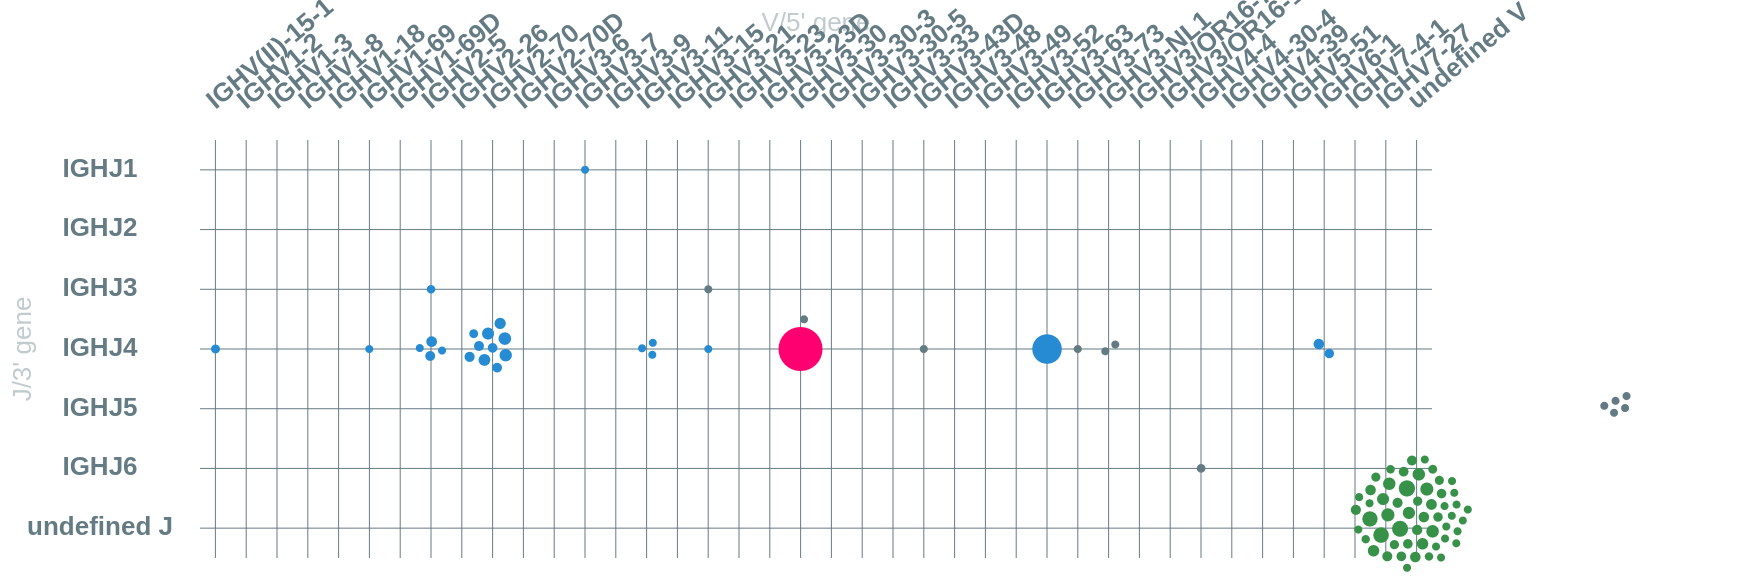
\includegraphics[width=1\textwidth]{images/diah_fr3_e1.png}
    \vspace{0.5cm}
    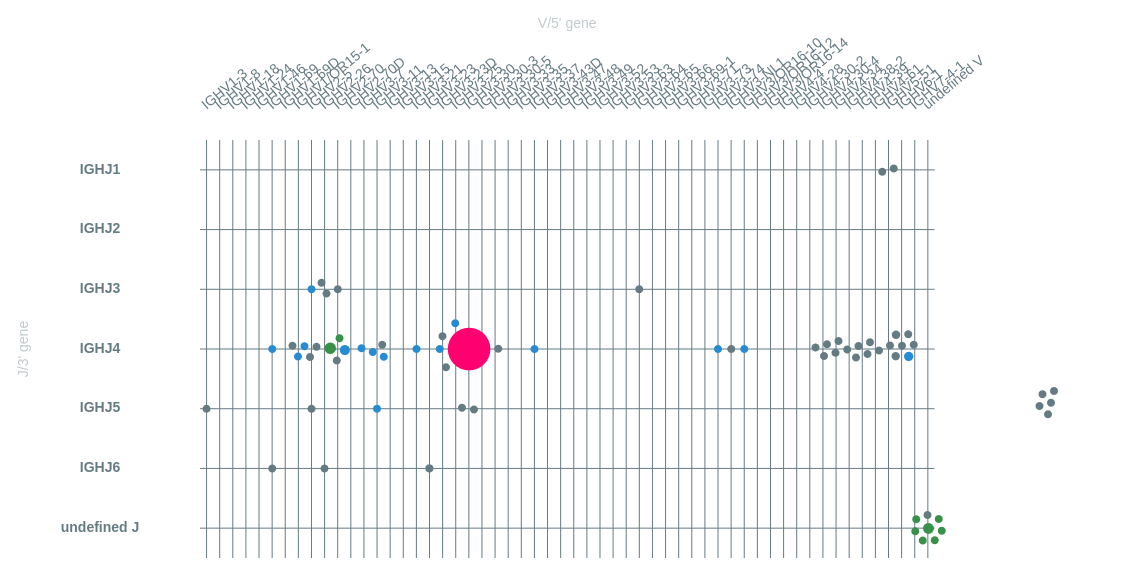
\includegraphics[width=1\textwidth]{images/diag_fr3_e-15.png}
    \caption{
        Répartition des clones identifiés en \gls{fr}3 avec une \textit{e-value} maximale de 1 (en haut)
        et de $10^{-15}$ (en bas) pour le patient 1 au diagnostic. \textcolor{Magenta}{Clone majoritaire (en rose)},
        \textcolor{ProcessBlue}{clones artéfactuels (en bleu)} et \textcolor{ForestGreen}{hors-cibles (en vert)}.
    }
    \label{fig:fr3-evalue}
\end{figure}

\subsection{Supression réversible de clonotypes}

Ainsi, une simple adaptation de la configuration de \textit{vidjil-algo} a
permis de réduire significativement la détection des clonotypes artéfactuels
liés aux séquences hors-cibles. Pour autant, certains de ces clonotypes
persistent dans les résultats, tandis que les dimères d'amorces demeurent en
grande partie non filtrés. Ces artéfacts fausseraient dès lors toute
quantification de la \gls{mrd} en sous-estimant le poids réel des véritables
clones. Il est possible via l'interface web de \textit{Vidjil} de masquer
temporairement certains clonotypes qui restent alors comptabilisés dans les
clones analysés, mais redeviennent visible à chaque rafraîchissement de la page
sans possibilité de sauvegarde. Il a donc été nécessaire de développer une
fonctionnalité permettant la suppression contrôlée des clonotypes, répondant
également aux attentes exprimées par d'autres utilisateurs.

\textbf{Exigences fonctionnelles définies pour le développement} :
\begin{itemize}
    \item Permettre à l'utilisateur de supprimer un ou plusieurs clonotypes de
          l'analyse.
    \item Rendre la suppression réversible, avec possibilité de restauration
          des clonotypes supprimés.
    \item Enregistrer les clonotypes supprimés lors de la sauvegarde des
          résultats.
    \item Exclure les clonotypes supprimés du total des clones analysés.
    \item Afficher de façon claire et explicite les clonotypes supprimés à
          l'utilisateur.
    \item Ne pas représenter les clonotypes supprimés dans les graphiques de
          répartition des clones.
\end{itemize}

\vspace{1em}

La mise en œuvre de ce cahier des charges implique principalement des
modifications de la partie client de \textit{Vidjil}, dont il est pertinent
d'en présenter brièvement l'architecture avant de détailler la solution
implémentée. Cette partie client est écrite en JavaScript natif et repose sur
58 scripts, dont 2 sont particulièrement importants pour cette nouvelle
fonctionnalité : \texttt{model.js} et \texttt{clone.js}. Le premier gère via un
objet \texttt{model} l'ensemble des attributs et méthodes nécessaires à la
gestion synchrone des données des clonotypes et métadonnées d'analyses, tandis
que le second gère des objets \texttt{clone} comprenant les données et méthodes
propres à chaque clonotype.

L'idée est donc la suivante : un nouvel attribut booléen \texttt{removed}
(initialisé par défaut sur la valeur \texttt{false}) est ajouté à l'objet
\texttt{clone} pour indiquer si le clonotype doit être supprimé ou non. Cet
attribut est contrôlé dans l'implémentation actuelle par un nouveau tag
utilisateur \texttt{removed\ clonotype}. 

Deux attributs \texttt{removed\_clones\_reads\_of\_active\_locus} et
\texttt{removed\_clones\_reads\_total} sont ajoutés à l'objet \texttt{model}
pour stocker le nombre de \textit{reads} des clonotypes supprimés indéxé par le
temps sous forme d'\textit{array} (tableau), respectivement pour le locus actif
et pour l'ensemble des loci (\autoref{algo:removed-reads}). Enfin la méthode
\texttt{getSize} de l'objet \texttt{clone}, ainsi que d'autres indicateurs du
nombre de \textit{reads} analysés sont modifiés pour soustraire de façon dynamique
du total des \textit{reads} le nombre de \textit{reads} des clonotypes supprimés.

\begin{algorithm}[H]
    \caption{Calcul des \textit{reads} des clonotypes supprimés à chaque temps}
    \label{algo:removed-reads}
    \KwIn{Nombre total de points temporels $T$}
    \KwOut{Vecteurs des \textit{reads} supprimés pour le locus sélectionné et au total}

    \SetKwData{RemovedReadsLocus}{removed\_clones\_reads\_of\_active\_locus}
    \SetKwData{RemovedReadsTotal}{removed\_clones\_reads\_total}
    \SetKwData{Germline}{germline}

    \tcp{Initialisation des variables}
    \RemovedReadsLocus $\leftarrow$ tableau de taille $T$ initialisé à $0$\;
    \RemovedReadsTotal $\leftarrow$ tableau de taille $T$ initialisé à $0$\;
    \Germline $\leftarrow$ liste vide\;

    \tcp{Récupération des loci sélectionnés}
    \For{chaque $i$ dans \texttt{system\_selected}}{
        Ajouter $i$ à \Germline\;
    }

    \tcp{Parcours des clones et mise à jour des reads supprimés}
    \For{chaque $j$ dans \texttt{clones}}{
        \If{\texttt{clones[$j$]} est marqué comme supprimé}{
            \For{$t$ de $0$ à $T-1$}{
                $reads \leftarrow$ \texttt{clones[$j$].getReads($t$)}\; \tcp{Reads du clone $j$ au temps $t$}
                \RemovedReadsTotal$[t] \mathrel{+}= reads$\;
                \If{\Germline contient \texttt{clones[$j$].get('germline')}}{
                    \RemovedReadsLocus$[t] \mathrel{+}= reads$\;
                }
            }
        }
    }

    Mise à jour des attributs \RemovedReadsLocus et \RemovedReadsTotal\
\end{algorithm}

En parallèle, des modifications de l'interface utilisateur ont été réalisées
afin d'afficher les clonotypes supprimés avec un format distinct permettant de
les différencier des autres. Ces clonotypes sont ainsi représentés en
transparence et barrés (\autoref{fig:removed-clonotypes}). Un clonotype virtuel
est également ajouté pour chaque locus afin de comptabiliser le pourcentage de
\textit{reads} supprimés par locus. Les clonotypes peuvent être restaurés en
supprimant le tag \texttt{removed clonotype}, cette information étant conservée
via ce même tag. Enfin, des tests unitaires ont été ajoutés pour garantir le
bon fonctionnement de cette fonctionnalité.

\begin{figure}[H]
    \begin{minipage}{0.65\textwidth}
        \centering
        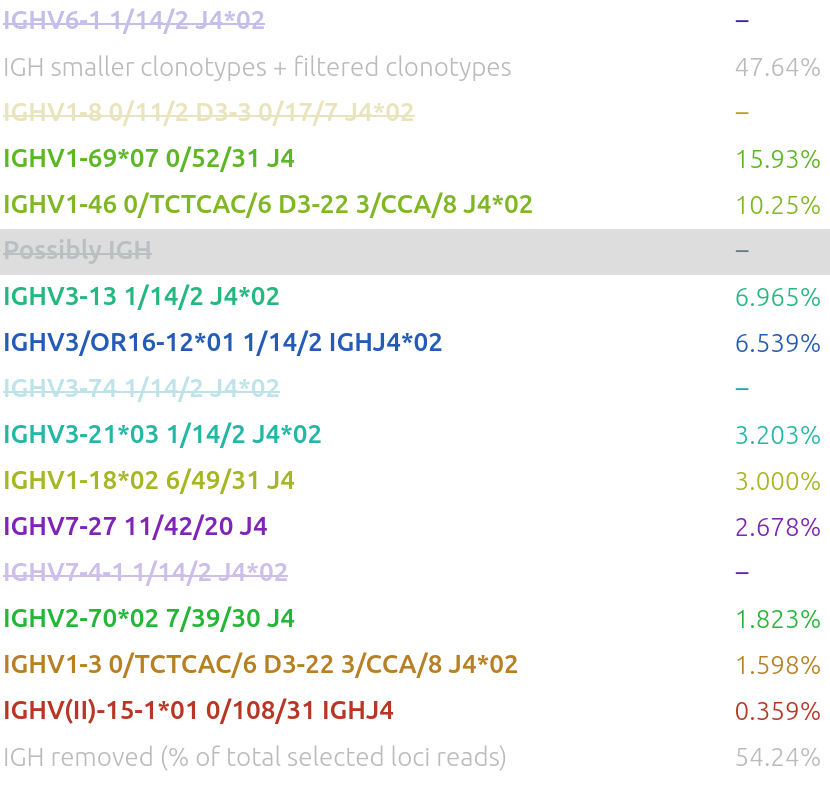
\includegraphics[width=1\textwidth]{images/removed_clonotypes.png}
    \end{minipage}
    \hfill
    \begin{minipage}{0.3\textwidth}
        \centering
        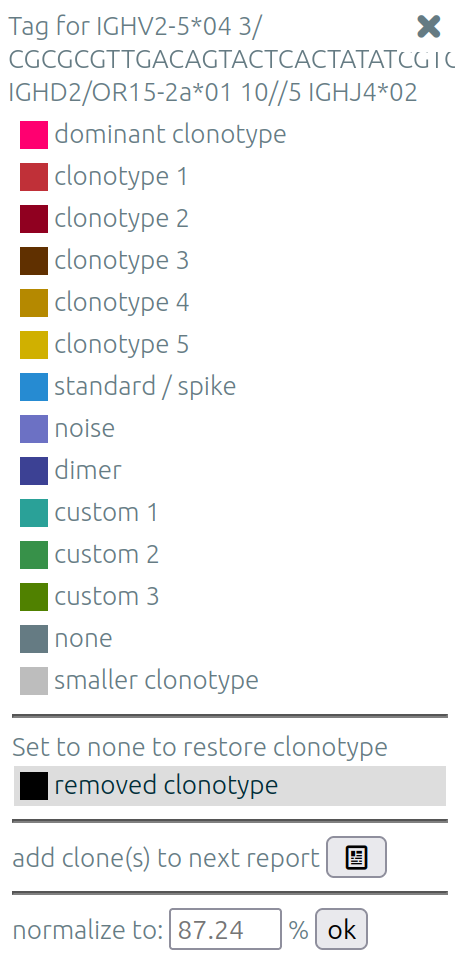
\includegraphics[width=01\textwidth]{images/tag_menu.png}
    \end{minipage}
    \caption{
        Capture d'écran de l'interface utilisateur de \textit{Vidjil} montrant les clonotypes supprimés.
        Les clonotypes sont affichés en transparence et barrés, et un clonotype virtuel est ajouté pour
        comptabiliser le pourcentage de \textit{reads} supprimés par locus (image de gauche).
        Menu des tags permettant de supprimer les clonotypes en ajoutant le tag \texttt{removed clonotype}
        (image de droite).
    }
    \label{fig:removed-clonotypes}
\end{figure}

\section{Etude de la MRD}

Il nous est maintenant possible de supprimer les clonotypes artéfactuels et
hors-cibles pour ne conserver que les réarrangements véritables lors de l'étude
de la \gls{mrd}, en parallèle des optimisations techniques réalisées.
L'évaluation de la \gls{mrd} est alors possible en comparant le réarrangement
clonal identifié au diagnostic à ceux présents au suivi, et nécessite de
pouvoir détecter avec précision des quantités très faibles de réarrangements
clonaux.

\subsection{Quantité de matériel nécessaire selon le seuil de détection analytique}

En premier lieu, il est nécessaire de s'assurer que le matériel de départ est
suffisant pour espérer détecter des quantités infimes de réarrangements
clonaux. Dans cette optique, il est possible de modéliser de façon assez simple
la question par un problème d'échantillonnage statistique. Si l'on considère
l'organisme comme la population ou chaque cellule représente un individu,
positif ou négatif (soit une cellule tumorale ou saine), avec une probabilité
$p$ qu'une cellule soit positive, en considérant chaque cellule comme un
échantillon indépendant, le nombre $N$ de cellules positives parmi $n$ cellules
analysées suivra une loi binomiale de paramètres $n$ et $p$. Dans les faits,
sachant que $p$ est très faible et $n$ assez elevé, on peut approximer la loi binomiale par une
loi de Poisson de paramètre $\lambda = n \cdot p$.

Ainsi, si l'on accepte un risque $\epsilon$ de ne pas détecter un réarrangement
clonal, en analysant $n$ cellules, malgré que le réarrangement soit présent
chez le patient, on peut écrire comme suit :

\begin{equation}
    N \sim \mathcal{B}(n, p) \approx \mathcal{P}(\lambda)
    \quad \text{avec} \quad \lambda = n \cdot p
\end{equation}

La probabilité de détecter au moins une cellule tumorale est donnée par :
\begin{equation}
    \mathbb{P}(N \geq 1) = 1 - \mathbb{P}(N = 0) = 1 - e^{-\lambda} = 1 - \varepsilon
\end{equation}

où $\varepsilon$ est le risque de non-détection fixé à l'avance (par exemple
$5\,\%$ pour un seuil de confiance de $95\,\%$). En pratique, la sensibilité
analytique des techniques de mesure de la \gls{mrd} ne permettent pas la
détection d'un événement unique, et il est plus juste de placer un seuil de
détection minimal $k$ \footnote{On confond ici volontairement pour des raisons
de simplicité le seuil de détection analytique $k_{\text{ana}}$, et $k$ le
seuil statistique, avec en pratique $k_{\text{ana}} \leq k$.} de l'ordre de 10 à
100 cellules positives :

\begin{equation}
    \mathbb{P}(N \geq k) = 1 - \sum_{i = 0}^{k-1} \frac{e^{-\lambda} \, \lambda^{i}}{i!} = 1 - \varepsilon
    \quad \text{soit} \quad \varepsilon(n,k \mid p) = \sum_{i = 0}^{k-1} \frac{e^{-np} \, (np)^{i}}{i!}
\end{equation}

On cherche donc a résoudre l'équation précédente en $n$, en sachant que $p$ est
inconnu dans les faits, mais estimé comme étant de l'ordre de $10^{-4}$ à
$10^{-8}$, valeur qui correspondrait à la proportion des cellules dites «
initiatrices de leucémie ». En faisant donc varier $p$ sur cet intervalle, avec
$\epsilon = 0.05$ et $k = 10$ puis $100$, on peut résoudre l'équation
précédente (de façon numérique et non algébrique, s'agissant d'une équation
transcendante). En considérant également la numération leucocytaire sanguine
comme étant de l'ordre de $5\,\text{G/L}$ et médullaire de $50\,\text{G/L}$, on
peut en déduire le volume minimal à prélever pour espérer détecter la \gls{mrd}
au seuil de confiance de $95\,\%$ (\autoref{tab:valeurs_n_volume}).

\begin{table}[H]
    \centering
    \caption{
        Nombre minimal de cellules $n$ et volume sanguin nécessaire pour différents $p$ et seuils $k$, avec $\varepsilon = 0.05$.
        Les volumes en \colorbox{mygreen}{vert} et \colorbox{myyellow}{jaune} sont analysables en pratique clinique, tandis que les
        volumes en \colorbox{myorange}{orange} et nuances de \colorbox{myred}{rouge} sont considérés comme trop élevés.
    }
    \label{tab:valeurs_n_volume}
    \begin{tabular}{c|cc|cc}
        \toprule
        \multirow{2}{*}{$p$} & \multicolumn{2}{c|}{$k = 10$} & \multicolumn{2}{c}{$k = 100$}                                                        \\
                             & $n$ (cellules)                & Volume (mL)                   & $n$ (cellules)        & Volume (mL)                  \\
        \midrule
        \multicolumn{5}{c}{Numération = $5\,\text{G/L}$}                                                                                            \\
        \midrule
        $10^{-4}$            & $1.57 \times 10^{5}$          & \cellcolor{mygreen}0.031      & $1.17 \times 10^{6}$  & \cellcolor{mygreen}0.234     \\
        $10^{-5}$            & $1.57 \times 10^{6}$          & \cellcolor{mygreen}0.314      & $1.17 \times 10^{7}$  & \cellcolor{myyellow}2.340    \\
        $10^{-6}$            & $1.57 \times 10^{7}$          & \cellcolor{myyellow}3.14      & $1.17 \times 10^{8}$  & \cellcolor{myorange}23.40    \\
        $10^{-7}$            & $1.57 \times 10^{8}$          & \cellcolor{myred}31.43        & $1.17 \times 10^{9}$  & \cellcolor{mydarkred}234.00  \\
        $10^{-8}$            & $1.57 \times 10^{9}$          & \cellcolor{mydarkred}314.29   & $1.17 \times 10^{10}$ & \cellcolor{mydeepred}2340.00 \\
        \midrule
        \multicolumn{5}{c}{Numération = $50\,\text{G/L}$}                                                                                           \\
        \midrule
        $10^{-4}$            & $1.57 \times 10^{5}$          & \cellcolor{mygreen}0.0031     & $1.17 \times 10^{6}$  & \cellcolor{mygreen}0.023     \\
        $10^{-5}$            & $1.57 \times 10^{6}$          & \cellcolor{mygreen}0.031      & $1.17 \times 10^{7}$  & \cellcolor{mygreen}0.234     \\
        $10^{-6}$            & $1.57 \times 10^{7}$          & \cellcolor{mygreen}0.31       & $1.17 \times 10^{8}$  & \cellcolor{myyellow}2.34     \\
        $10^{-7}$            & $1.57 \times 10^{8}$          & \cellcolor{myyellow}3.14      & $1.17 \times 10^{9}$  & \cellcolor{myorange}23.40    \\
        $10^{-8}$            & $1.57 \times 10^{9}$          & \cellcolor{myred}31.43        & $1.17 \times 10^{10}$ & \cellcolor{mydarkred}234.00  \\
        \bottomrule
    \end{tabular}
\end{table}

Ainsi, pour un seuil de détection à $10^{-5}$ avec 100 cellules minimum, il est
nécessaire de prélever au moins 3 mL de sang et 10 fois moins de moelle, ce qui
correspond à une quantité d'environ 500 ng d'ADN (A vérfier avec Aurélie +
correspondance en reads). On remarque également que des seuils de détection
inférieurs à $10^{-6}$ sont jusqu'à présent inatteignables, nécessitant des
volumes de prélèvement pouvant atteindre plusieurs litres.

TO BE CONTINUED

\subsection{Quantification de la MRD}

Résultats leader et fr3 sur les 5 couples après modifications température, +
spike in, quantification, normalisation cellules

\subsection{Détection de la MRD sur les échantillons cliniques}

Comparaison résultats CMF, etc .